%
% File naaclhlt2018.tex

\documentclass[11pt,a4paper]{article}
\usepackage[hyperref]{naaclhlt2018}
\usepackage{times}
\usepackage{latexsym}
\usepackage{tikz}
\usepackage{tikz-dependency}
\usepackage[warn]{textcomp}
\usepackage{subcaption}

\usepackage{url}

\usepackage{etoolbox}

\makeatletter
\patchcmd\@combinedblfloats{\box\@outputbox}{\unvbox\@outputbox}{}{%
   \errmessage{\noexpand\@combinedblfloats could not be patched}%
}%
 \makeatother


\usetikzlibrary{shapes,shapes.misc}

%\aclfinalcopy % Uncomment this line for the final submission
%\def\aclpaperid{***} %  Enter the acl Paper ID here

%\setlength\titlebox{5cm}
% You can expand the titlebox if you need extra space
% to show all the authors. Please do not make the titlebox
% smaller than 5cm (the original size); we will check this
% in the camera-ready version and ask you to change it back.

\title{Deep Multitask Learning for Transition-Based DAG Parsing}

\author{Daniel Hershcovich$^{1,2}$ \\
  \\\And
  Omri Abend$^2$ \\
  $^1$The Edmond and Lily Safra Center for Brain Sciences \\
  $^2$School of Computer Science and Engineering \\
  Hebrew University of Jerusalem \\
  \texttt{\{danielh,oabend,arir\}@cs.huji.ac.il}
  \\\And
  Ari Rappoport$^2$
}

\date{}

\begin{document}
\maketitle
\begin{abstract}
  We train a transition-based DAG parser on multiple semantic parsing tasks.
  In a multitask setting, we observe improvements on a low-resource task,
  Universal Conceptual Cognitive Annotation parsing, using other schemes
  as auxiliary tasks.
  Despite various divergences between semantic representation schemes,
  there are many commonalities both structurally and in terms of semantic content.
  We convert these schemes into a unified format and investigate how
  the similarity between different tasks is related to the contribution of
  using one as an auxiliary task for another.
\end{abstract}

\section{Introduction}\label{sec:introduction}

Following increased interest in semantic representation,
recent developments in natural language processing have focused on semantic parsing, including
Abstract Meaning Representation parsing \cite[AMR;][]{banarescu2013abstract,damonte-17,11099},
Semantic Dependency Parsing \cite[SDP;][]{oepen2015semeval,P17-1186},
Universal Conceptual Cognitive Annotation parsing \cite[UCCA;][]{abend2013universal,hershcovich2017a},
and frame-semantic parsing \cite{gildea2002automatic,swayamdipta2017frame,ringgaard2017sling},
among others.
In parallel, syntactic dependency parsers are becoming more accurate.
Specifically, parsing to Universal Dependencies \cite[UD;][]{nivre2016universal,dozat2016deep}
reflects learning syntactic structure in a language-universal way.

Semantic parsing often requires parsers that can handle a general directed acyclic graph (DAG)
structure.
While each of these representation schemes has its own set of distinctions it focuses on,
much of the semantic content is shared between many of them \cite{abend2017state}.
Given the success of multitask learning models in various tasks
\cite{collobert2008unified,luong2015multi,ruder2017overview}
including parsing specifically
\cite{Zhang2016StackpropagationIR,P17-1186,swayamdipta2017frame,guo2016exploiting}
we propose a multitask transition-based semantic parser.


\begin{figure*}
\begin{subfigure}[t]{0.5\textwidth}
  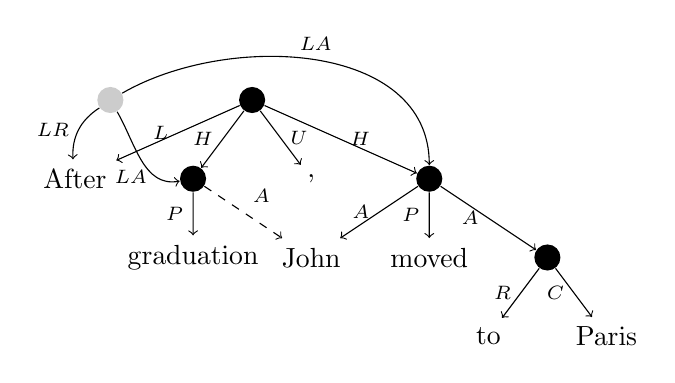
\begin{tikzpicture}[level distance=10mm, ->]
    \node (ROOT) [fill=black, circle] {}
      child {node (After) {After} edge from parent node[left] {\scriptsize $L$}}
      child {node (graduation) [fill=black, circle] {}
      {
        child {node {graduation} edge from parent node[left] {\scriptsize $P$}}
      } edge from parent node[left] {\scriptsize $H$} }
      child {node {,} edge from parent node[right] {\scriptsize $U$}}
      child {node (moved) [fill=black, circle] {}
      {
        child {node (John) {John} edge from parent node[left] {\scriptsize $A$}}
        child {node {moved} edge from parent node[left] {\scriptsize $P$}}
        child {node [fill=black, circle] {}
        {
          child {node {to} edge from parent node[left] {\scriptsize $R$}}
          child {node {Paris} edge from parent node[left] {\scriptsize $C$}}
        } edge from parent node[left] {\scriptsize $A$} }
      } edge from parent node[right] {\scriptsize $H$} }
      ;
    \draw[dashed,->] (graduation) to node [auto] {\scriptsize $A$} (John);
    \node (LKG) at (-1.8,0) [fill=black!20, circle] {};
    \draw[bend right] (LKG) to node [auto, left] {\scriptsize $LR$} (After);
    \draw (LKG) to[out=-60, in=190] node [below] {\scriptsize $LA\quad$} (graduation);
    \draw (LKG) to[out=30, in=90] node [above] {\scriptsize $LA$} (moved);
  \end{tikzpicture}
  \caption{UCCA graph.
  The dashed edge is remote.
  The gray node and its outgoing edges represent linkage between the two scenes.
  Pre-terminal nodes and edges are omitted for brevity.}
  \label{fig:original_example_ucca}
\end{subfigure}
~
\begin{subfigure}[t]{0.5\textwidth}
  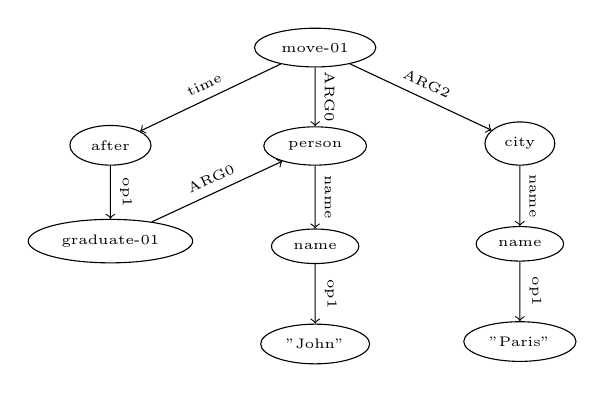
\begin{tikzpicture}[level distance=15mm, ->,
      every node/.append style={sloped,anchor=south,auto=false,font=\tiny},
      level 1/.style={sibling distance=26mm}]
    \node (ROOT) [draw=black,ellipse] {move-01}
      child {node [draw=black,ellipse] {after}
      {
            child {node (graduation) [draw=black,ellipse] {graduate-01} edge from parent node {op1} }
      } edge from parent node {time} }
      child {node (John) [draw=black,ellipse] {person}
      {
        child {node [draw=black,ellipse] {name}
        {
            child {node [draw=black,ellipse] {"John"} edge from parent node {op1} }
        } edge from parent node {name} }
      } edge from parent node {ARG0} }
      child {node [draw=black,ellipse] {city}
      {
        child {node [draw=black,ellipse] {name}
        {
            child {node [draw=black,ellipse] {"Paris"} edge from parent node {op1} }
        } edge from parent node {name} }
      } edge from parent node {ARG2} }
      ;
      \draw (graduation) to node {ARG0} (John);
  \end{tikzpicture}
  \captionof{figure}{AMR graph.
  The text tokens are not part of the graph, and must be matched to
  concepts and constants by alignment.
  Variables are represented by their concepts.}
  \label{fig:original_example_amr}
\end{subfigure}

\begin{subfigure}[t]{0.5\textwidth}
    \begin{dependency}[text only label, label style={above}, font=\small]
    \begin{deptext}[column sep=.1em,ampersand replacement=\^]
    After \^ graduation \^ , \^ John \^ moved \^ to \^ Paris \\
    \end{deptext}
        \depedge{1}{2}{ARG2}
        \depedge{5}{4}{ARG1}
        \depedge[edge unit distance=2ex]{1}{5}{ARG1}
        \deproot{5}{top}
        \depedge[edge unit distance=4ex, edge start x offset=-1ex]{5}{7}{ARG2}
        \depedge[edge start x offset=1ex]{6}{5}{ARG1}
        \depedge{6}{7}{ARG2}
    \end{dependency}
  \captionof{figure}{SDP graph (in the DM formalism).
  The graph contains multiple roots: ``After'', ``moved'' and ``to''.
  One of the roots is marked as \textit{top}: ``moved''.
  Punctuation is not included in the graph as it is non-content-bearing.}
  \label{fig:original_example_sdp}
\end{subfigure}
~
\begin{subfigure}[t]{0.5\textwidth}
    \begin{dependency}[text only label, label style={above}, font=\small]
    \begin{deptext}[column sep=.1em,ampersand replacement=\^]
    After \^ graduation \^ , \^ John \^ moved \^ to \^ Paris \\
    \end{deptext}
        \depedge{2}{1}{case}
        \depedge{4}{3}{punct}
        \depedge{5}{4}{nsubj}
        \depedge{2}{5}{obl}
        \depedge{7}{6}{case}
        \deproot{5}{root}
        \depedge{5}{7}{obl}
    \end{dependency}
  \captionof{figure}{UD tree.
  Each word has exactly one head, and there is a single root.
  Edge labels correspond to syntactic relations.}
  \label{fig:original_example_ud}
\end{subfigure}

\caption{Example for each representation scheme whose parsing task we handle.}
\label{fig:original_examples}
\end{figure*}

\section{Tasks}\label{sec:tasks}

In this work, we focus on representation schemes providing a \textit{whole-sentence} analysis,
that is, annotating a graph connecting all (content) words in a sentence.
This is in contrast to ``shallow'' semantic parsing,
such as Semantic Role Labeling
\cite[SRL;][]{Palmer:05,gildea2002automatic,swayamdipta2017frame,ringgaard2017sling},
or parsing to logical forms.
We consider four target representations: UCCA, AMR, SDP and UD.
Figure~\ref{fig:original_examples} shows an example graph for each scheme,
annotating the sentence ``After graduation, John moved to Paris''.

\subsection{Universal Conceptual Cognitive Annotation}\label{sec:ucca}

UCCA \cite{abend2013universal} represents the semantics of natural language utterances
as directed acyclic graphs (DAGs), where terminal nodes (nodes without children)
correspond to the text tokens and
non-terminal nodes to semantic or cognitive entities or relations.
Edges are labeled, indicating the role of a child in the relation the parent represents.
Nodes and edges may belong to one of several \textit{layers}, each layer corresponding
to a ``module'' of semantic distinctions.
UCCA's \textit{foundational layer} mostly covers predicate-argument
structure, coordination and multi-word expressions.
The \textit{linkage} layer covers relations between events, including temporal and discourse relations
(exemplified by the gray node and its outgoing edges in Figure~\ref{fig:original_example_ucca}).

UCCA's guidelines distinguish between \textit{primary} edges, corresponding to the roles explicit
in the text, and \textit{remote} edges (such as the dashes edge in
Figure~\ref{fig:original_example_ucca}), corresponding to implicit relations.
Primary edges form a tree structure in each layer,
whereas the remote edges enable reentrancy (a DAG structure).


\subsection{Abstract Meaning Representation}\label{sec:amr}

AMR \cite{banarescu2013abstract}
is a semantic representation that embeds annotations related
to named entity recognition, semantic role labeling, word
sense disambiguation and co-reference resolution.
AMRs are rooted and directed graphs, in which both nodes and edges are labeled.
Most AMRs are DAGs, although cycles are permitted.
AMR was targeted in the SemEval 2017 shared task \cite{may2017semeval}.

As can be seen in Figure~\ref{fig:original_example_amr}, text tokens are not part
of the AMR graph, which connects only concepts (from a pre-defined set)
and constants (which may be strings or numbers).
During the process of parsing from plain text to AMR,
the tokens are aligned to graph nodes,
a process referred to as concept identification.
AMR datasets already contain automatically aligned graphs.

\subsection{Broad-Coverage Semantic Dependency Parsing}\label{sec:sdp}

SDP \cite{oepen2014semeval,oepen2015semeval,oepen2016towards}
is a set related tasks, targeted in two SemEval shared tasks.
They correspond to four semantic representation schemes, referred to as
DM, PAS, PSD and CCD, representing
predicate-argument relations between content-bearing words in a sentence.
All are based on semantic formalisms whose annotations have been
converted into bilexical dependencies:
they are labeled directed graphs whose nodes are all text tokens.
Edges are labeled, encoding semantic relations between the tokens.
Non-content-bearing tokens, such as punctuation,
may be left out of the analysis (see Figure~\ref{fig:original_example_sdp}),
but the subgraph restricted to content-bearing tokens is connected.
Graphs containing cycles have been removed from the SDP datasets.

We consider one of the three formalisms used in the SemEval shared task:
the DM (DELPH-IN MRS) representation, which comes
from DeepBank \cite{flickinger2012deepbank},
manually-corrected parses from the LinGO
English Resource Grammar \cite{copestake2000open}.
LinGO is a head-driven phrase
structure grammar \cite[HPSG; ][]{pollard1994head}
with minimal recursion semantics \cite{copestake2005minimal}.

\subsection{Universal Dependencies}\label{sec:ud}

The fourth formalism we consider is not a semantic representation, but
is instead acknowledged as a syntactic annotation scheme.
UD \cite{nivre2016universal,11234/1-2515} has become
the dominant dependency representation for
annotating treebanks in a large variety of languages,
aiming for cross-linguistically consistent treebank
annotations for as many languages as possible.
Representations are bilexical trees, with edge labels representing
syntactic relations between the text tokens.

We use UD as an auxiliary task,
similar to syntactic scaffolding employed by \cite{swayamdipta2017frame}.
Thanks to its annotation in multiple languages, we can use it as an auxiliary task
for UCCA parsing in German and French (see \S\ref{sec:multilingual}).


\begin{figure*}
\begin{subfigure}[t]{0.5\textwidth}
    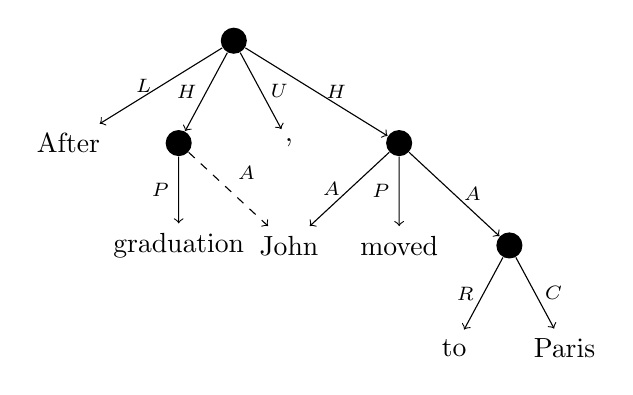
\begin{tikzpicture}[level distance=13mm, sibling distance=14mm, ->,
        every circle node/.append style={fill=black}]
      \tikzstyle{word} = [font=\rmfamily,color=black]
      \node (ROOT) [circle] {}
        child {node (After) [word] {After} edge from parent node[left] {\scriptsize $L$}}
        child {node (graduation) [circle] {}
        {
          child {node [word] {graduation} edge from parent node[left] {\scriptsize $P$}}
        } edge from parent node[left] {\scriptsize $H$} }
        child {node [word] {,} edge from parent node[right] {\scriptsize $U$}}
        child {node (moved) [circle] {}
        {
          child {node (John) [word] {John} edge from parent node[left] {\scriptsize $A$}}
          child {node [word] {moved} edge from parent node[left] {\scriptsize $P$}}
          child {node [circle] {}
          {
            child {node [word] {to} edge from parent node[left] {\scriptsize $R$}}
            child {node [word] {Paris} edge from parent node[right] {\scriptsize $C$}}
          } edge from parent node[right] {\scriptsize $A$} }
        } edge from parent node[right] {\scriptsize $H$} }
        ;
      \draw[dashed,->] (graduation) to node [auto] {\scriptsize $A$} (John);
    \end{tikzpicture}
  \caption{Converted UCCA graph.
  Linkage nodes and edges are removed, but otherwise the original UCCA graph is preserved.}
  \label{fig:converted_example_ucca}
\end{subfigure}
~
\begin{subfigure}[t]{0.5\textwidth}
  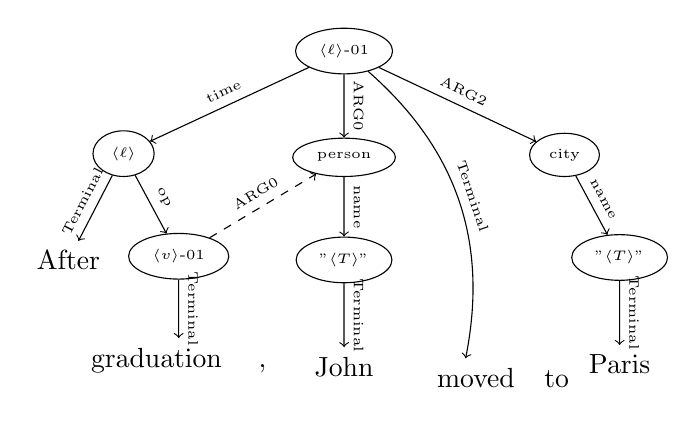
\begin{tikzpicture}[level distance=16mm, ->,
      every node/.append style={sloped,anchor=south,auto=false,font=\tiny},
      level 1/.style={sibling distance=28mm},
      level 2/.style={sibling distance=14mm},
      level 3/.style={sibling distance=12mm}]
    \tikzstyle{word} = [font=\rmfamily,color=black]
    \node (ROOT) [draw=black,ellipse] {$\langle \ell \rangle$-01}
      child {node [draw=black,ellipse] {$\langle \ell \rangle$}
      {
            child {node [word] {After} edge from parent node {\tiny Terminal}}
            child {node (graduation) [draw=black,ellipse] {$\langle v \rangle$-01}
            {
              child {node [word] {graduation \quad ,} edge from parent node {\tiny Terminal}}
            } edge from parent node {op} }
      } edge from parent node {time} }
      child {node (John) [draw=black,ellipse] {person}
      {
        child {node [draw=black,ellipse] {"$\langle T \rangle$"}
        {
          child {node [word] {John} edge from parent node {\tiny Terminal}}
        } edge from parent node {name} }
      } edge from parent node {ARG0} }
      child {node [draw=black,ellipse] {city}
      {
        child {node {}
        {
            child {node [word] (moved) {\quad moved} edge from parent [draw=none]}
            child {node [word] {to} edge from parent [draw=none]}
        } edge from parent [draw=none]}
        child {node [draw=black,ellipse] {"$\langle T \rangle$"}
        {
          child {node [word] {Paris} edge from parent node {\tiny Terminal}}
        } edge from parent node {name} }
      } edge from parent node {ARG2} }
      ;
      \draw[bend left] (ROOT) to node {\tiny Terminal} (moved);
      \draw[dashed] (graduation) to node {ARG0} (John);
  \end{tikzpicture}
  \captionof{figure}{Converted AMR graph, with
  text tokens added according to the alignments, and
  pre-terminals included to show node labels.
  The placeholders $\langle \ell \rangle, \langle v \rangle$ and $\langle T \rangle$
  correspond to the lemma, related verb form and surface form, respectively.
  Numeric suffixes of \textit{op} relations were removed,
  and names collapsed.}
  \label{fig:converted_example_amr}
\end{subfigure}

\begin{subfigure}[t]{0.5\textwidth}
  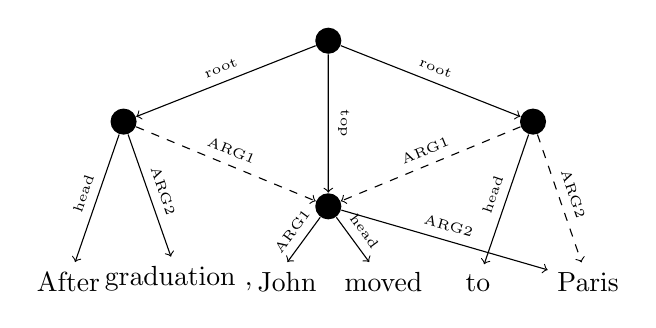
\begin{tikzpicture}[level distance=12mm, ->,
      every node/.append style={sloped,anchor=south,auto=false,font=\tiny},
      level 1/.style={sibling distance=26mm},
      level 2/.style={sibling distance=14mm}]
    \tikzstyle{word} = [font=\rmfamily,color=black]
    \node (ROOT) [fill=black,circle] {}
      child {node (after) [fill=black,circle] {}
      {
        child {node [draw=none] {}
        {
          child {node [word] (after_word) {After} edge from parent [draw=none]}
        } edge from parent [draw=none] }
        child {node [draw=none] {}
        {
          child {node [word] (graduation) {graduation ,} edge from parent [draw=none]}
        } edge from parent [draw=none] }
      } edge from parent node {root}}
      child {node [draw=none] {}
      {
        child {node (moved) [fill=black,circle] {}
        {
          child {node [word] {\quad John} edge from parent node {ARG1}}
          child {node [word] {moved} edge from parent node {head}}
        } edge from parent [draw=none] }
      } edge from parent [draw=none] }
      child {node (to) [fill=black,circle] {}
      {
        child {node [draw=none] {}
        {
            child {node [word] (to_word) {to} edge from parent [draw=none]}
          } edge from parent [draw=none] }
          child {node [draw=none] {}
        {
          child {node [word] (Paris) {Paris} edge from parent [draw=none]}
        } edge from parent [draw=none] }
      } edge from parent node {root}}
      ;
      \draw (ROOT) to node {top} (moved);
      \draw (after) to node {head} (after_word);
      \draw (after) to node {ARG2} (graduation);
      \draw[dashed] (after) to node {ARG1} (moved);
      \draw[dashed] (to) to node {ARG1} (moved);
      \draw (to) to node {head} (to_word);
      \draw (moved) to node {ARG2} (Paris);
      \draw[dashed] (to) to node {ARG2} (Paris);
  \end{tikzpicture}
  \captionof{figure}{Converted SDP graph (in the DM formalism).
  Intermediate non-terminal nodes are introduced, including \textit{head} edges.
  Reentrant edges are marked as remote (dashed).}
  \label{fig:converted_example_sdp}
\end{subfigure}
~
\begin{subfigure}[t]{0.5\textwidth}
  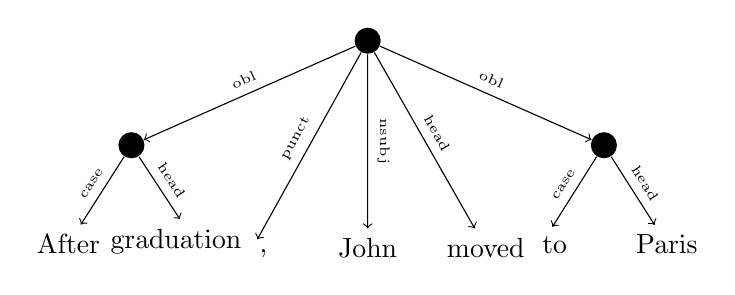
\begin{tikzpicture}[level distance=15mm, ->,
      every node/.append style={sloped,anchor=south,auto=false,font=\tiny},
      level 1/.style={sibling distance=15mm},
      level 2/.style={sibling distance=16mm}]
    \tikzstyle{word} = [font=\rmfamily,color=black]
    \node (ROOT) [fill=black,circle] {}
      child {node (after) [fill=black,circle] {}
      {
        child {node [word] {After} edge from parent node {case}}
        child {node [word] {graduation \quad\quad} edge from parent node {head}}
      } edge from parent node {obl}}
      child {node {}
      {
        child {node [word] (comma) {\quad ,} edge from parent [draw=none]}
      } edge from parent [draw=none]}
      child {node {}
      {
        child {node [word] (John) {John} edge from parent [draw=none]}
      } edge from parent [draw=none]}
      child {node {}
      {
        child {node [word] (moved) {moved} edge from parent [draw=none]}
      } edge from parent [draw=none]}
      child {node (to) [fill=black,circle] {}
      {
          child {node [word] {\quad to} edge from parent node {case}}
          child {node [word] {Paris} edge from parent node {head}}
      } edge from parent node {obl}}
      ;
      \draw (ROOT) to node {punct} (comma);
      \draw (ROOT) to node {nsubj} (John);
      \draw (ROOT) to node {head} (moved);
  \end{tikzpicture}
  \captionof{figure}{Converted UD graph.
  As in SDP, intermediate non-terminals and \textit{head} edges are introduced.
  The graph is actually a tree, as was the original bilexical graph.}
  \label{fig:converted_example_ud}
\end{subfigure}

\caption{Graphs in unified DAG format.
Pre-terminal nodes are omitted for brevity, except in AMR.}
\label{fig:converted_examples}
\end{figure*}


\section{Unified DAG format}\label{sec:conversion}

To be able to tackle the four tasks presented in \S\ref{sec:tasks} using a single model,
we develop a conversion algorithm for each scheme,
to convert it into a unified DAG format.
In this format, the graph is a rooted DAG, and the text tokens are terminal nodes.
Edges are labeled, and nodes are optionally labeled too (to support AMR parsing).
All edges entering terminals bear the \textit{Terminal} label.
As in the UCCA format,
graph edges are divided into \textit{primary} and \textit{remote} edges,
where the primary edges form a tree (all nodes have at most one primary parent,
and the root has none).
The remote edges enable reentrancy, and thus together with them the graph
is in general a DAG and not necessarily a tree.
Not all non-terminals must have terminal descendants.
Non-terminals with an empty terminal yield are called \textit{implicit}.
Figure~\ref{fig:converted_examples} shows examples for converted graphs.

Converting UCCA into the unified format consists simply of removing linkage nodes
and edges (see Figure~\ref{fig:converted_example_ucca}).
To convert bilexical dependencies (SDP and UD) into the unified DAG format,
we add a pre-terminal for each terminal,
and then attach the pre-terminals according to the original dependency edges.
We add an additional level with a \textit{head} edge to avoid terminal and non-terminal siblings
(see Figure~\ref{fig:converted_example_sdp} and Figure~\ref{fig:converted_example_ud}).
Since SDP allows multiple roots, we attached the corresponding non-terminals as children of
the single converted graph root, with the \textit{root} edge label.
Top nodes are labeled with \textit{top} instead.
In case of reentrancy, an arbitrary parent is marked as primary, and the rest as remote
(denoted as dashed edges in Figure~\ref{fig:converted_examples}).

In the conversion from AMR, non-terminals are already present and do not need to be introduced.
However, alignments and node labels must be handled
(see Figure~\ref{fig:converted_example_amr}).

\subsection{Alignments}
Since alignment to the text tokens is not part of the AMR graph,
we introduce the alignments as edges in conversion.
We use automatically aligned AMR graphs provided in the dataset (see \S\ref{sec:data}),
and attach each node with a \textit{Terminal} edge to each of the terminals it is aligned to.

\subsection{Node label sparsity}
To reduce the number of unique node labels, we use the alignments to introduce
placeholders in the labels.
For example, a node labeled \textit{move-01} aligned to the terminal \textit{moved} will
be instead labeled $\langle \ell \rangle$\textit{-01},
where $\langle \ell \rangle$ is a placeholder for the token's lemma.
In this way we reduce the number of node labels in the dataset from tens of thousands to 7300,
of which 2000 occur only once and are treated as unknown.
We use similar placeholders for the token's text and capitalized text,
negation, verb, noun and adjective form
(from a pre-defined lexicon), and Wikipedia concept.
We use DBpedia Spotlight to wikify concepts \cite{isem2013daiber}.
In addition, we omit all variable identifiers and instead label nodes directly with their concept.
This is similar to the delexicalization employed by \citet{buys2017oxford}.

\subsection{Edge label sparsity}
Another sparsity issue is with ordinal relations, such as \textit{op1}, \textit{op2}, etc.
Since the order of relations is annotated according to the order of text tokens,
the numeric index is redundant and is thus removed.
We keep the numeric suffixes when they are meaningful, e.g. in \textit{ARG0}, \textit{ARG1}, etc.

\subsection{Names}
Named entities in AMR are expressed by \textit{name} relations and nodes, with
a child for each token in the name, with relations labeled \textit{op1}, \textit{op2}, etc.
We instead collapse this subgraph to a single node whose label is the concatenation of the
name tokens, replaced by a $\langle T \rangle$ placeholder if aligned.



\section{Transition-based universal parser}\label{sec:model}

The unified DAG format introduced in \S\ref{sec:conversion}
exhibits reentrancy, discontinuity and non-terminal nodes.
To learn to parse representations in this format,
we extend TUPA \cite{hershcovich2017a},
a transition-based parser that supports these structural properties,
originally developed for UCCA.
TUPA's general transition system allows parsing any aligned DAG structure with labeled edges.
To support AMR parsing, we add transitions to handle node labels and unaligned nodes
(see \S\ref{sec:transition_set}).

Transition-based parsers \cite{Nivre03anefficient} apply \textit{transitions}
incrementally to an internal state defined by
a buffer $B$ of remaining tokens and nodes,
a stack $S$ of incomplete nodes,
and a labeled graph $G$ of constructed nodes and edges.
When the parsing process is finished, the graph $G$ is the final output.
A classifier is used at each step to select the next transition based on features
encoding the current state.
During training, an oracle creates training instances for the classifier,
based on gold-standard annotations.


\subsection{Transition set}\label{sec:transition_set}
Given a sequence of tokens $w_1, \ldots, w_n$,
we predict a graph $G$ in the unified format over the sequence.
Parsing starts with the root node on the stack,
and the input tokens in the buffer.

The original TUPA transitions are
the standard \textsc{Shift} and \textsc{Reduce} operations,
\textsc{Node$_X$} for creating a new non-terminal node and an $X$-labeled edge,
\textsc{Left-Edge$_X$} and \textsc{Right-Edge$_X$} to create a new primary $X$-labeled edge,
\textsc{Left-Remote$_X$} and \textsc{Right-Remote$_X$} to create a new remote $X$-labeled edge,
\textsc{Swap} to handle discontinuous nodes,
and \textsc{Finish} to mark the state as terminal.

In addition, we add the \textsc{Implicit} transition, creating a new non-terminal
node as a \textit{child} of the current stack top rather than as its parent,
and transitions to
label nodes in the stack, \textsc{Label$_1$} and \textsc{Label$_2$},
labeling the stack top and one node to its left, respectively.

Although UCCA contains implicit units, that is, units without
any terminals as descendents,
the standard evaluation for UCCA \cite{abend2013universal} is span-based and
ignores these nodes.
For this reason we do not include this transition when parsing UCCA.
However, for AMR we do include it, as AMRs may contain unaligned concepts,
which correspond to implicit nodes in the unified format.
These are essential for AMR parsing, for which evaluation is done
by graph matching, using the Smatch algorithm \cite{cai2013smatch}.

The reason for including \textsc{Label$_2$} is that often a node's
label can be determined more accurately only after attaching its children,
which may require it to be the second node on the stack.
To keep the overall number of transitions manageable,
the node label itself is not part of the transition's identity,
instead being selected by a separate classifier.

\subsection{Classifier}\label{sec:classifier}
We experiment with two different models for the parser in the single-task case:
(1) a linear classifier with sparse features, trained with the averaged structured perceptron algorithm
\cite{Coll:04} and \textsc{MinUpdate} \cite{goldberg2011learning},
and (2) a bidirectional LSTM feature extractor with dense embeddings as inputs,
combined with a feedforward network and a softmax layer for classification.

For all classifiers, inference is performed greedily,
and training is done with an oracle that provides a set of all possible labels at a given state
(but only valid transitions may be taken during training).

\begin{figure}[t]
   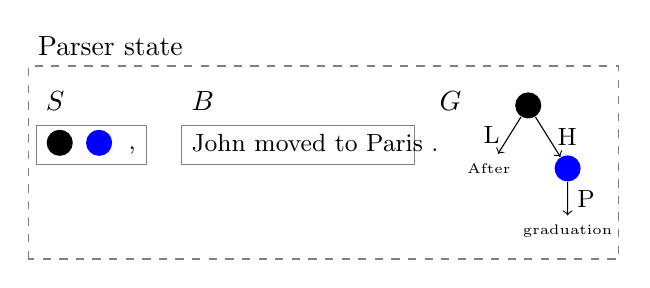
\begin{tikzpicture}[level distance=8mm, sibling distance=1cm]
   \node[anchor=west] at (0,1.5) {Parser state};
   \draw[color=gray,dashed] (0,-1.2) rectangle (7.5,1.25);
   \draw[color=gray] (.1,0) rectangle (1.5,.5);
   \node[anchor=west] at (.1,.8) {$S$};
   \node[fill=black, circle] at (.4,.275) {};
   \node[fill=blue, circle] at (.9,.275) {};
   \node[anchor=west] at (1.15,.175) {\small ,};
   \draw[color=gray] (1.95,0) rectangle (4.9,.5);
   \node[anchor=west] at (1.95,.8) {$B$};
   \node[anchor=west] at (1.95,.275) {\small John moved to Paris .};
   \node[anchor=west] at (5.1,.8) {$G$};
   \node[fill=black, circle] at (6.35,.75) {}
     child {node  {\tiny After} edge from parent [->] node[left] {\small L}}
     child {node [fill=blue, circle] {}
     {
       child {node {\tiny graduation} edge from parent [->] node[right] {\small P}}
     } edge from parent [->] node[right] {\small H} };
   \end{tikzpicture}
   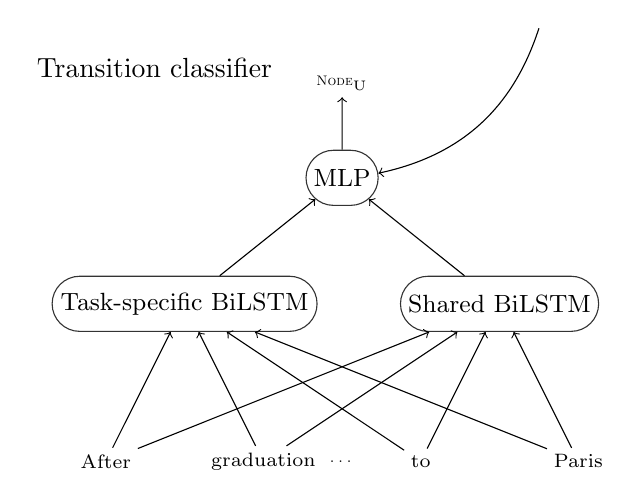
\begin{tikzpicture}[->]
   \node[anchor=west] at (0,6) {Transition classifier};
   \tiny
   \tikzstyle{main}=[rounded rectangle, minimum size=7mm, draw=black!80, node distance=12mm]
   \node[main] (specific) at (2,3) {\small Task-specific BiLSTM};
   \node[main] (shared) at (6,3) {\small Shared BiLSTM};
   \foreach \i/\word in {1/{After},3/{graduation},5/{to},7/{Paris}} {
       \node (x\i) at (\i,1) {\scriptsize \word};
       \path (x\i) edge (specific);
       \path (x\i) edge (shared);
   }
    \node (x4) at (4,1) {\ldots};
    \node[main] (mlp) at (4,4.6) {\small MLP};
    \path (specific) edge (mlp);
    \path (shared) edge (mlp);
    \coordinate (state) at (6.5,6.5);
    \path (state) edge [bend left] (mlp);
    \node (transition) at (4,5.8) {\textsc{Node}\textsubscript{U}};
    \path (mlp) edge (transition);
   \end{tikzpicture}
   \caption{Illustration of the model.
      Top: parser state (stack, buffer and intermediate graph).
      Bottom: NN architecture.
      Vector representations for the input tokens is computed
      by two multilayer BiLSTMs:
      one specific to the current task, and one shared among all tasks.
      The resulting vectors for specific tokens are concatenated with
      embedding and numeric features from the parser state
      (for existing edge labels, number of children, etc.),
      and fed into the MLP for selecting the next transition.}
   \label{fig:model}
\end{figure}

In addition to the features used by \citet{hershcovich2017a},
for AMR we add node label features according to
previously predicted node labels for node in specific locations in the parser state.

Lemmas, POS tags, syntactic dependency labels and named entities are extracted using spaCy
\cite{spacy2}.\footnote{\url{https://spacy.io}}
We use the categorical cross-entropy objective function and optimize the
NN classifiers with stochastic gradient descent (SGD).
We use 250K word vectors from fastText \cite{bojanowski2016enriching}, pretrained over Wikipedia.
The neural network is implemented using DyNet \cite{neubig2017dynet}.\footnote{\url{https://dynet.io}}
Hyperparameter settings are listed in Table~\ref{tab:hyperparams}.

\begin{table}
\begin{tabular}{l|ccc}
& Sparse & NN \\
\hline
\multicolumn{3}{l}{\footnotesize Embedding dimensions} \\
external word & & 300 \\
word & & 200 \\
POS tag & & 20 \\
syntactic dep. & & 10 \\
edge label & & 20 \\
punctuation & & 1 \\
action & & 3 \\
node labels & & 20 \\
\hline
\multicolumn{3}{l}{\footnotesize Other parameters} \\
$\textsc{MinUpdate}$ & 5 \\
initial learning rate & 1 & 1 \\
learning rate decay & 0.1 & 0.01 \\
MLP \#layers & & 2 \\
MLP layer dim. & & 50 \\
LSTM \#layers & & 2 \\
LSTM layer dim. & & 500 \\
word dropout & & 0.2 \\
dropout & & 0.4 \\
weight decay & & $10^{-5}$ \\
mini-batch size & & 100
\end{tabular}
\caption{Hyperparameter settings.\label{tab:hyperparams}}
\end{table}


\subsection{Constraints}

As each annotation scheme has different constraints on the allowed graphs,
we declared these constraints separately for each task.
During training and parsing, the constraint set corresponding to the task is
selected and applied to the parser state.

Some constraints are task-specific, while some are generic.
For example, in UCCA, a terminal may only have one parent.
In UD, every node may only have one parent.
In AMR, a concept corresponding to a PropBank frame may only core arguments defined for the frame.

As an example for a generic constraint, nodes that have already been swapped
should never be swapped again.
To implement this constraint efficiently, we define a \textit{swap index}
for each node, which is assigned when the node is created.
At parse start, only the root node and terminals exist.
We assign the root a swap index of 0, and for each terminal, its swap index
is its position in the text (starting at 1).
Whenever a node is created as a result of a \textsc{Node} or \textsc{Implicit}
transition, we assign its swap index to be the mean of the stack top and buffer
head's swap indices.


\subsection{Unlabeled parsing}\label{sec:unlabeled}

We extend the parser to support unlabeled parsing by simply removing all labels from
\textsc{Edge}, \textsc{Remote}, \textsc{Node} and \textsc{Implicit} actions output by the oracle.
This results in a much smaller output dimension, but of course only unlabeled evaluation is
meaningful in this case.



\section{Multitask transition-based parsing}\label{sec:multitask}

Since the same model can be applied to different tasks, we can train it jointly on multiple tasks.
In this section we focus on the NN model.
Rather than sharing the whole set of parameters (and getting a mix of action labels as a result),
we share only part of the model.
Specifically, in addition to the task-specific input-encoding bidirectional LSTM,
we use a shared bidirectional LSTM. The outputs of both LSTMs are concatenated and
fed into the task-specific MLP, in a manner similar to \citet{P17-1186}.

Multitask learning is particularly beneficial for improving on tasks with small training data.
As UCCA has a relatively small corpus (see \S\ref{sec:data}),
we focus on UCCA parsing and treat AMR, SDP and UD parsing
as auxiliary tasks, creating a unified corpus by shuffling all sentences from all datasets together,
but using only the score on the UCCA development set as the criterion for early stopping.

\subsection{Unlabeled parsing for auxiliary tasks}\label{sec:unlabeled_aux}

Preliminary experiments showed that simply training the model in this manner yield no improvement
on the UCCA development set, when compared to training on the UCCA corpus alone.
We hypothesized that the auxiliary tasks were actually difficult enough on their own,
and could not provide enough backpropagation signal to the shared parameter set.
We thus decided to use unlabeled parsing for all auxiliary tasks, while still doing labeled UCCA parsing.


\section{Experiments}\label{sec:experiments}

We perform various experiments to evaluate the benefit of each auxiliary task to UCCA parsing.
First, we train the parser separately on each task.
Next, we train it to parser UCCA in a multitask setting, where AMR, SDP and UD are used as
auxiliary tasks. Following previous work, we use the same hyperparameter settings
as for the single-task case \cite{N16-1179,P16-2038,C16-1013,C16-1059,C16-1179,E17-1005}.

\subsection{Data}\label{sec:data}

For UCCA, we use the English Wikipedia corpus \cite{abend2013universal},
and the \textit{Twenty Thousand Leagues Under the Sea} corpus \cite[20K leagues;][]{sulem2015conceptual},
annotated in English, French and German.
For AMR, we use LDC2016E25, used in SemEval 2017 \cite{may2017semeval}.
For SDP, we use data for the DM target representation from SemEval 2015 \cite{oepen2015semeval}.
For Universal Dependencies, we use UD v2.1 \cite{11234/1-2515}.
Table~\ref{tab:corpora} shows the size of each corpus.

Since the UCCA corpus is disproportionally small in comparison to the auxiliary task corpora,
simply training on all training data would create a model that is geared toward the auxiliary tasks.
To overcome this problem,
at each training iteration we sample a subset of the training set for each auxiliary task.
The subset size is identical to the UCCA training set size.

\begin{table}
\begin{tabular}{lcc}
Corpus & \# Tokens & \# Sentences \\
\textbf{UCCA} \\
Wiki & 158433 & 5225 \\
20K Leagues: \\
English & 12339 & 506 \\
French & 12929 & 547 \\
German & 113524 & 4764 \\
\textbf{UD} \\
English & 408466 & 24276 \\
French & 1067840 & 40102 \\
German & 308107 & 16590 \\
\textbf{AMR} \\
LDC2016E25 & 708701 & 39260 \\
\textbf{SDP} \\
SemEval 2015 & 802717 & 35657 \\
\end{tabular}
\caption{Size of each corpus.\label{tab:corpora}}
\end{table}


\subsection{Evaluation}\label{sec:evaluation}

As each scheme has its own evaluation metric, we evaluate them separately.
For UCCA, we evaluate labeled precision, recall and F1 on primary and remote edges.
For UD, we use LAS F1.
For AMR, we use Smatch \cite{cai2013smatch}.
For SDP, we use labeled precision, recall and F1.


\subsection{Results}\label{sec:results}




\subsection{Single-task parsing}\label{sec:results_single}

To evaluate the conversion and parsing algorithm on each task, we report the result
of training the parser on each task separately.
In this case we perform labeled parsing for all tasks, and use the whole training set.
The results for single-task parsing, when evaluated on the development set for each task,
are shown in Table~\ref{tab:single}.



\begin{table}
\begin{tabular}{llccc}
\textbf{UCCA} & & \textbf{LP} & \textbf{LR} & \textbf{LF} \\
Sparse & \small Primary & 63.4 & 64.3 & 63.8 \\
       & \small Remote & 17 & 14.3 & 15.5 \\
NN & \small Primary & 74.5 & 74.9 & 74.7 \\
       & \small Remote & 49.2 & 50.5 & 49.8 \\
\hline
\textbf{UD} & \small LAS & & & \textbf{F1} \\
Sparse & & & & 64.8 \\
NN & & & & 80.1 \\
\hline
\textbf{AMR} & \small Smatch & \textbf{P} & \textbf{R} & \textbf{F1} \\
Sparse & & 55 & 53.7 & 54.4 \\
NN & & 64.9 & 64.3 & 64.6 \\
\hline
\textbf{SDP} & & \textbf{LP} & \textbf{LR} & \textbf{LF} \\
Sparse & & 55.2 & 51.4 & 53.2 \\
NN & & 76 & 75.4 & 75.7
\end{tabular}
\caption{Single-task results on the English development set for each task.\label{tab:single}}
\end{table}


\subsection{Multitask parsing}\label{sec:results_multi}

Next, we focus on UCCA parsing, and assess the contribution of each auxiliary task
and combinations thereof, by evaluating on the UCCA development set.
As mentioned in \S\ref{sec:unlabeled_aux}, we train on all auxiliary tasks as unlabeled tasks.
The results for multitask parsing are shown in Table~\ref{tab:multi}.

\begin{table}
\begin{tabular}{lccc|ccc}
& \multicolumn{3}{c|}{Primary} & \multicolumn{3}{c}{Remote} \\
& \textbf{LP} & \textbf{LR} & \textbf{LF} & \textbf{LP} & \textbf{LR} & \textbf{LF} \\
\small AMR & 73.5 & 73.5 & 73.5 & 52.6 & 43.9 & 47.9\\
\small UD & 73.4 & 73.2 & 73.3 & 50.5 & 46.7 & 48.5 \\
\small SDP & 74.3 & 73.2 & 73.7 & 52.9 & 51.7 & 52.3 \\
\small SDP+UD & 73.4 & 72.7 & 73.1 & 48.5 & 51.7 & 50.1 \\
\small AMR+UD & 73.3 & 73.6 & 73.4 & 51.2 & 45.8 & 48.4 \\
\small AMR+SDP & 74.2 & 73.3 & 73.8 & 53 & 52.6 & 52.8 \\
\small all & 73.7 & 73.3 & 73.5 & 50.6 & 49.2 & 49.9
\end{tabular}
\caption{Multitask results on the UCCA English Wiki development set.
The UCCA Wiki training set is used in each case, in addition to the training
set for the specified task.\label{tab:multi}}
\end{table}


\subsection{Multilingual parsing}\label{sec:multilingual}

To investigate the contribution of multitask training on an even smaller UCCA training set,
we experiment with the French and German \textit{20K Leagues} UCCA corpora.
The results are given in Table~\ref{tab:multilingual}.
The contribution of multitask learning is substantial in this case:
although the sparse classifier has an advantage on small datasets
(the NN classifier does not get even a single edge right on the tiny French dataset),
when coupled with UD parsing as an auxiliary task, the NN classifier surpasses it
in both languages.
This shows that a small UCCA training corpus may suffice, as long as it is complemented by
a large training corpus in an auxiliary task in the same language.

\begin{table}
\begin{tabular}{lccc|ccc}
& \multicolumn{3}{c|}{Primary} & \multicolumn{3}{c}{Remote} \\
\textbf{German} & \textbf{LP} & \textbf{LR} & \textbf{LF} & \textbf{LP} & \textbf{LR} & \textbf{LF} \\
\multicolumn{3}{l}{Single-task:} \\
\small Sparse & 67.4 & 65.5 & 66.4 & 24.1 & 2.9 & 5.1 \\
\small NN & 54.2 & 38.4 & 45 & 35 & 17.3 & 23.1 \\
\multicolumn{3}{l}{Multitask (UCCA + UD):} \\
\small NN & 74.6 & 74.1 & 74.4 & 66 & 13.6 & 22.5 \\
\hline
\textbf{French} \\
\multicolumn{3}{l}{Single-task:} \\
\small Sparse & 60.8 & 59.2 & 60 & 7.1 & 3.8 & 4.9 \\
\small NN & 100 & 0 & 0 & 100 & 0 & 0 \\
\multicolumn{3}{l}{Multitask (UCCA + UD):} \\
\small NN & 64.4 & 64.4 & 64.4 & 36.4 & 7.5 & 12.5
\end{tabular}
\caption{Single-task and multitask results on the UCCA 20K Leagues development set in German and French.\label{tab:multilingual}}
\end{table}



\section{Related work}\label{sec:related_work}

In general, multitask learning involves optimizing more than one loss function \cite{ruder2017overview}.
However, in our case, the loss function has the same form across all tasks.
The same architecture and inference algorithm are applied to multiple annotation formats and datasets,
and only some of the parameters are shared between them: this is hard parameter sharing.

Multitask learning is often used in NLP, both as regularization when little training data is available,
and as an alternative to the pipeline approach, to avoid error propagation
\cite{collobert2008unified}.
Multitask learning has been applied to semantic parsing, including
semantic dependency parsing \cite{P17-1186} and
frame semantic parsing \cite{swayamdipta2017frame}.
In transition-based parsing, multitask learning has been applied to
tagging and parsing \cite{bohnet2012transition,Zhang2016StackpropagationIR},
lexical and syntactic analysis \cite{constant-nivre:2016:P16-1,more2016joint},
and semantic-syntactic analysis \cite{swayamdipta-EtAl:2016:CoNLL,henderson2013multilingual}.


\section{Discussion}\label{sec:discussion}

\subsection{Common edges}\label{sec:common}

An important factor in the success of multitask learning is the commonalities between the tasks
\cite{E17-2026,E17-1005}.
In fact, this is why we decided to convert the auxiliary tasks into UCCA-like format for
multitask training in the first place.
To get a sense of the similarity between the converted formats and actual UCCA graphs,
we perform unlabeled evaluation of the conversion results and gold-standard UCCA.
However, since we do not have a gold-standard corpus annotated for both UCCA and another scheme,
we use leading parsers for the auxiliary formats and apply them to the text of the
UCCA development set. The results are listed in Table~\ref{tab:common}.

\begin{table}
\begin{tabular}{lccc|ccc}
& \multicolumn{3}{c|}{Primary} & \multicolumn{3}{c}{Remote} \\
& \textbf{UP} & \textbf{UR} & \textbf{UF} & \textbf{UP} & \textbf{UR} & \textbf{UF} \\
AMR \\
SDP \\
UD \\
\end{tabular}
\caption{Unlabeled UCCA evaluation of each scheme after parsing the UCCA development
set and converting to the unified DAG format.\label{tab:common}}
\end{table}


\bibliography{references}
\bibliographystyle{acl_natbib}

\end{document}
